\begin{tikzpicture}
  % z-plane: the ellipse |z + mu zbar| = 1 for mu = 0.4 e^{i pi/3}
  \begin{scope}
    \draw[gray, ->] (-2.1,0) -- (2.1,0) node[right, font=\small, black] {$x$};
    \draw[gray, ->] (0,-2.1) -- (0,2.1) node[above, font=\small, black] {$y$};
    \draw[gray, dashed] (210:2) -- (30:2);
    \draw[gray, dashed] (300:2) -- (120:2);
    \draw[blue, thick, rotate=120] (0,0) ellipse (1.667 and 0.714);
    \draw[red, thick, ->] (0,0) -- (30:0.714);
    \draw[red, thick, ->] (0,0) -- (120:1.667);
    \node[font=\scriptsize, right] at (30:0.8) {$\tfrac{1}{1+|\mu|}$};
    \node[font=\scriptsize, left] at (120:1.2) {$\tfrac{1}{1-|\mu|}$};
    \node[font=\small] at (0,-2.5) {$z$-plane: $|z+\mu\bar z|=1$};
  \end{scope}
  \draw[->, thick] (2.5,0.4) -- node[above, font=\small] {$h(z)=z+\mu\bar z$} (4.6,0.4);
  % h-plane: the unit circle
  \begin{scope}[xshift=7cm]
    \draw[gray, ->] (-2.1,0) -- (2.1,0);
    \draw[gray, ->] (0,-2.1) -- (0,2.1);
    \draw[gray, dashed] (210:2) -- (30:2);
    \draw[gray, dashed] (300:2) -- (120:2);
    \draw[blue, thick] (0,0) circle (1);
    \draw[red, thick, ->] (0,0) -- (30:1);
    \draw[red, thick, ->] (0,0) -- (120:1);
    \node[font=\small] at (0,-2.5) {$h$-plane: $|h|=1$};
  \end{scope}
\end{tikzpicture}
